%auto-ignore
\chapter[Longitudinal Neuroanatomical Progression of PCA]{Longitudinal Neuroanatomical Progression of Posterior Cortical Atrophy}
\label{chapter:pca}

This chapter outlines the clinically applied part of my PhD, which focused on modelling the progression of Posterior Cortical Atrophy using already developed methods. The content of this chapter is based on the neuroimaging results from the joint publication below, where I've re-written most of the text for this thesis. I performed all the neuroimaging work: image pre-processing, statistical analysis with EBM and DEM, and the interpretation of the results. The data from table \ref{tab:pcaDemographics} was gathered by Nicholas Firth. Splitting of PCA patients into cognitively-defined subgroups was done by Silvia Primativo. Details in section \ref{sec:pcaParticipants} regarding patient recruitment, patient numbers, clinical diagnosis and pathological confirmation along with image acquisition details from section \ref{sec:pcaImageAcq} were taken from our joint publication.


\section{Publications}

\begin{itemize}
 \item N. C. Firth*, S. Primativo*, R. V. Marinescu*, T. J. Shakespeare, A. Suarez-Gonzalez, M. Lehmann, A. Carton, D. Ocal, I. Pavisic, R. W. Paterson, C. F. Slattery, A. J. M. Foulkes, B. H. Ridha, E. Gil-Néciga, N. P. Oxtoby, A. L. Young, M. Modat, M. J. Cardoso, S. Ourselin, N. S. Ryan, B. L. Miller, G. D. Rabinovici, E. K. Warrington, M. N. Rossor, N. C. Fox, J. D. Warren, D. C. Alexander, J. M. Schott, K. X. X. Yong\^{} and S. J. Crutch\^{}, Longitudinal neuroanatomical and cognitive progression of posterior cortical atrophy, Brain, 2019. (*) joint first authors (\^{}) joint senior authors
 
 In the above manuscript, I preprocessed all the imaging data, performed the modelling and statistical analysis of all the imaging data, and created the figures, tables and diagrams (including statistical tests in the supplementary). I also drafted the section of the results which was related to the imaging results. Other authors recruited patients, collected the data, performed the analysis of cognitive tests, and helped draft the initial version of the manuscript. 

 \item R. V. Marinescu, A. L. Young, Neil P. Oxtoby, N. C. Firth, M. Lorenzi, A. Eshaghi, V. Wottschel, M. J. Cardoso, M. Modat, K. X. X. Yong, S. Primativo, N. C. Fox, M. Lehmann, T. J. Shakespeare, S. J. Crutch, D. C. Alexander, A data-driven comparison of the progression of brain atrophy in Posterior Cortical Atrophy and Alzheimer's disease, AAIC poster, 2016.

 \item R. V. Marinescu, S. Primativo, A. L. Young, N. P. Oxtoby, N. C. Firth, A. Eshaghi, S. Garbarino, J. M. Cardoso, K. Yong, N. C. Fox, M. Lehmann, T. J. Shakespeare, S. J. Crutch, D. C. Alexander, Analysis of the heterogeneity of Posterior Cortical Atrophy: Data-driven Model Predicts Distinct Atrophy Patterns for three different Cognitive Subgroups, AAIC poster, 2017 
\end{itemize}


\section{Introduction}

% Posterior Cortical Atrophy
Posterior Cortical Atrophy (PCA), already described in section \ref{sec:bckPca}, is a progressive neurodegenerative syndrome causing predominantly visuospatial and visuoperceptual impairments \cite{crutch2012posterior}. In order to understand complex disease mechanisms underlying PCA, and design efficient clinical trials for finding treatments of PCA, we need to be able to accurately estimate the temporal progression of atrophy in PCA and contrast it with typical AD (tAD). Previous neuroimaging studies of PCA have shown more atrophy in the superior parietal, occipital and posterior temporal regions as compared to typical AD \cite{lehmann2011cortical, whitwell2007imaging}. However, these studies are all cross-sectional and cannot map the continuous longitudinal progression of the disease. One longitudinal study of PCA \cite{lehmann2012global} showed widespread gray matter loss in both PCA and tAD, but the numbers were small (17 PCA and 16 tAD) and the time interval was short (1 year). Larger longitudinal studies are therefore required to robustly estimate longitudinal progression patterns of PCA as compared to tAD. Moreover, a second aspect that needs to be clarified is the heterogeneity within PCA itself. Some studies have so far reported three dominant subgroups: primary visual (the striate cortex, caudal), parietal (dorsal) and occipito-temporal (ventral) \cite{ross1996progressive,galton2000atypical}. However, evidence for the existence of these groups is mainly limited to individual case reports \cite{ross1996progressive,galton2000atypical} and no previous study looked at the temporal progression of brain atrophy in such subgroups.

The aim of this study is to estimate the progression of MRI brain volumes in PCA as compared to tAD. We used the event-based model (EBM, section \ref{sec:bckEbm}) and the differential equation model (DEM, section \ref{sec:bckDem}) to estimate the progression of brain volumes in 361 individuals (117 PCA, 106 tAD and 138 controls) from three centres in the UK, Spain and US. We also use the event-based model to estimate the progression of atrophy in three cognitively-defined PCA subgroups. Compared to previous studies, our study is the first comprehensive study of atrophy progression in PCA. We also provide the first glimpse into the early progression of atrophy within PCA subgroups. 


\section{Methods}

\subsection{Participants}
\label{sec:pcaParticipants}

% Number of patients, clinical diagnosis, pathological confirmation.
117 patients with PCA were recruited from three specialist centres: 100 from the Dementia Research Centre (DRC) UK, 9 patients from the University Hospital Virgen del Rocio (HUVR) Memory disorders Unit, Spain and 8 patients from the University of California San Francisco (UCSF) Memory and Aging Center, USA. All PCA participants met two widely-accepted Tang-Wai et al. \cite{tang2004clinical} and Mendez, Ghajarania \& Perryman \cite{mendez2002posterior} criteria. Participants had no clinical features of other neurodegenerative disorders (e.g. visual hallucinations, pyramidal signs), hence fulfilling the criteria for PCA-pure \cite{crutch2017consensus}. 106 tAD patients and 138 healthy controls recruited from the DRC UK were also used for this study. tAD subjects all met criteria for \emph{probable} AD \cite{mckhann2011diagnosis}. Available pathological and molecular analyses for the patients (45/117 = 38\% for PCA, 49/106  = 46\% for tAD) all indicated AD pathology. 

% Neuroimaging and cognitive
Of all the study participants, 270 had undergone at least one T1 MRI scan and 216 at least one cognitive assessment. Available neuroimaging and neuropsychology data, stratified by the number of visits, are shown in table \ref{tab:pcaDemographics}. PCA, tAD and healthy controls were age-matched (65.44 $\pm$ 7.51 for PCA, 65.67 $\pm$ 7.57 for tAD and 63.13 $\pm$ 5.94 for controls). The gender proportion was as follows: 39\% male for PCA, 62\% male for tAD and 50\% male for controls. PCA and tAD subjects had a similar level of impairment as measured by MMSE scores at first assessment: 20.88 $\pm$ 5.17 for PCA, 19.58 $\pm$ 5.08 for tAD and 29.02 $\pm$ 0.98 for controls. 

\newcommand{\tabwidth}{1cm}

\begin{table}
\centering
\begin{tabular}{c | c c c | c c c}
 & \multicolumn{3}{c|}{\textbf{Imaging}} & \multicolumn{3}{c}{\textbf{Neuropsychology}}\\
\textbf{Visits} & \textbf{Number} & \textbf{Age} & \textbf{Visit Interval} & \textbf{Number} & \textbf{Age} & \textbf{Visit Interval} \\
\multicolumn{7}{c}{}\\
\multicolumn{7}{c}{\textbf{PCA (n=117)}}\\
\hline
All & 89 & 63.52 $\pm$ 6.91 & N/A & 109 & 64.49 $\pm$ 7.54 & N/A \\
≥2 & 46 & 62.11 $\pm$ 6.52 & 1.03 $\pm$ 0.47 & 70 & 63.64 $\pm$ 7.32 & 1.18 $\pm$ 0.48 \\
≥3 & 31 & 62.75 $\pm$ 6.5 & 0.99 $\pm$ 0.47 & 45 & 62.73 $\pm$ 7.26 & 1.15 $\pm$ 0.45 \\ 
≥4 & 15 & 61.46 $\pm$ 4.44 & 0.86 $\pm$ 0.31 & 20 & 63.19 $\pm$ 7.00 & 1.14 $\pm$ 0.40 \\ 
≥5 & 9 & 61.73 $\pm$ 4.06 & 0.81 $\pm$ 0.33 & 7 & 59.44 $\pm$ 4.84 & 1.06 $\pm$ 0.45 \\
≥6 & 2 & 62.35 $\pm$ 1.65 & 0.83 $\pm$ 0.24 & 2 & 57.22 $\pm$ 3.49 & 1.02 $\pm$ 0.35 \\
\multicolumn{7}{c}{}\\
\multicolumn{7}{c}{\textbf{tAD (n=106)}} \\ 
\hline
All & 66 & 66.39 $\pm$ 8.58 & N/A & 58 & 65.68 $\pm$ 7.57 & N/A \\
≥2 & 37 & 66.84 $\pm$ 8.83 & 0.83 $\pm$ 1.46 & 28 & 64.58 $\pm$ 7.08 & 1.35 $\pm$ 0.56 \\ 
≥3 & 21 & 71.0 $\pm$ 6.97 & 0.53 $\pm$ 0.39 & 5 & 66.08 $\pm$ 2.78 & 1.26 $\pm$ 0.43 \\ 
≥4 & 14 & 70.89 $\pm$ 6.33 & 0.47 $\pm$ 0.33 & 0 & N/A & N/A \\
≥5 & 4 & 72.08 $\pm$ 4.81 & 0.49 $\pm$ 0.33 & 0 & N/A & N/A \\ 
≥6 & 1 & 79.9 $\pm$ 0.0 & 0.58 $\pm$ 0.40 & 0 & N/A & N/A \\
\multicolumn{7}{c}{}\\
\multicolumn{7}{c}{\textbf{Controls (n=138)}} \\
\hline
All & 115 & 61.87 $\pm$ 10.43 & N/A & 49 & 63.12 $\pm$ 5.90 & N/A \\
≥2 & 50 & 61 $\pm$ 12.01 & 0.79 $\pm$ 0.66 & 18 & 60.00 $\pm$ 5.87 & 0.91 $\pm$ 0.27 \\
≥3 & 28 & 65.75 $\pm$ 5.96 & 0.66 $\pm$ 0.52 & 0 & N/A & N/A \\
≥4 & 17 & 66.82 $\pm$ 4.88 & 0.45 $\pm$ 0.28 & 0 & N/A & N/A \\
≥5 & 8 & 66.11 $\pm$ 4.83 & 0.44 $\pm$ 0.25 & 0 & N/A & N/A \\
≥6 & 0 & N/A & N/A & 0 & N/A & N/A \\

\end{tabular}
\caption[Demographic details for participants in the PCA study]{Demographic details for participants in the PCA study. Number of participants (n), mean and standard deviation age of participants at baseline visit and mean and standard deviation of visit interval is shown per number of visits. }
\label{tab:pcaDemographics}
\end{table}

\begin{table}
\centering
\begin{tabular}{C{5cm}|c|c|c|c|c|c}
%\toprule
 & \multicolumn{2}{C{3.5cm}|}{\textbf{Vision subgroup (n=30)}} & \multicolumn{2}{C{3.5cm}|}{\textbf{Space subgroup (n=30)}} & \multicolumn{2}{C{3.5cm}}{\textbf{Object subgroup (n=29)}} \\
%\cline{2-7}
& n & mean (std) & n & mean (std) & n & mean (std)\\
\hline
MMSE &  29 &     22.38 (5.19) &  28 &    19.54 (4.10) &  29 &     21.90 (5.62) \\
Age &  30 &     64.23 (7.72) &  30 &    63.26 (7.44) &  29 &     65.05 (8.48) \\
Gender (\%male)	&	30 & 16\% &	30 &	46\% &	29 & 41\% \\
PAL &   6 &     15.00 (5.66) &   5 &     5.60 (6.18) &   8 &     10.75 (7.14) \\
Digitspan forwards &  17 &      6.76 (2.86) &  27 &     6.15 (2.46) &  24 &      7.08 (2.36) \\
Digitspan backwards &  16 &      3.88 (1.69) &  28 &     2.89 (1.42) &  23 &      3.78 (2.08) \\
GDA addition &  17 &      1.59 (1.94) &  22 &     0.55 (1.41) &  19 &      1.95 (2.84) \\
GDA subtraction &  17 &      0.76 (1.16) &  22 &     0.23 (0.67) &  19 &      1.84 (2.87) \\
\hline
\textbf{Memory} & & & & & \\
SRMT faces &  18 &     18.78 (4.13) &  25 &    18.88 (4.30) &  20 &     18.10 (3.95) \\
SRMT words &  30 &     21.70 (2.88) &  30 &    19.43 (3.45) &  29 &     20.38 (2.73) \\
\hline
\textbf{Visual processing} & & & & & \\
Shape detection (VOSP) &  28 &     14.43 (3.29) &  29 &    17.17 (2.24) &  28 &     17.18 (2.42) \\
Shape discrimination &  28 &     12.96 (3.18) &  28 &    15.21 (3.45) &  28 &     16.14 (2.68) \\
Crowding &  22 &      6.68 (4.23) &  28 &     9.07 (2.34) &  28 &      8.71 (2.23) \\
\hline
\textbf{Space Perception} & & & & & \\
Number location &  29 &      2.10 (2.66) &  29 &     2.07 (2.69) &  28 &      4.68 (2.83) \\
Dot counting (n correct) &  29 &      4.03 (3.27) &  29 &     3.93 (3.15) &  29 &      6.93 (2.64) \\
A cancellation (time) &  28 &    73.90 (20.24) &  29 &   82.25 (13.95) &  28 &    62.68 (22.65) \\
A cancellation (n misses) &  29 &      5.76 (5.33) &  29 &     4.00 (4.36) &  29 &      3.62 (4.77) \\
\hline
\textbf{Object perception} & & & & & \\
Object decision &  30 &      9.77 (4.51) &  30 &    12.63 (3.95) &  29 &     10.03 (4.13) \\
Fragmented letters &  23 &      3.57 (4.99) &  29 &     6.34 (5.25) &  27 &      5.19 (5.72) \\
Unusual views &  20 &      3.05 (3.97) &  25 &     6.16 (5.03) &  22 &      3.36 (3.95) \\
Usual views &  20 &      9.65 (6.42) &  25 &    15.16 (4.89) &  22 &     12.59 (5.58) \\
\hline
Memory -- visual processing composite score discrepancy &  30 &   -28.90 (16.82) &  30 &   14.26 (20.33) &  29 &    11.93 (14.79) \\
Space -- object composite score discrepancy  &  30 &    -1.62 (26.91) &  30 &   23.06 (16.93) &  29 &   -17.70 (16.30) \\
%\bottomrule
\end{tabular}
\caption[Baseline population demographics for PCA subgroups]{Baseline population demographics and neuropsychological data for PCA subgroups. For every neuropsychological test, we report the number of participants with available data (n) and the mean and standard deviation of the available measures.}
\label{tab:pcaSubgrDemographics}
\end{table}



% PCA subgroups
For analysing the heterogeneity within PCA, we split the dataset into three groups based on performance on a suite of cognitive tests. For each subject we computed the following composite tests by summing up scores from individual tests:
\begin{itemize}
 \item Early visual processing: shape detection, shape discrimination and crowding
 \item Visuoperceptual processing: object decision, fragmented letters, usual and unusual views.
 \item Visuospatial processing: number location, dot counting and A cancellation (time -- cut off at 90s)
 \item Episodic memory: short recognition memory test (sRMT) for words and faces
\end{itemize}

The score for each of the four categories was computed by standardising each of the sub-scores on a 0-100 scale, corresponding to the minimum and maximum values obtained by the participants, and then taking the average within each category. The subjects were then classified into three groups. The worst 1/3 of subjects (n=30) on the early visual processing tests as compared to the memory tests (i.e. difference between early visual and memory tests) were assigned to the vision subgroup. The remaining 2/3 of participants were split into two groups based on the difference between visuoperceptual and visuospatial tasks: subjects with space $<$ object performance (n=30) were assigned to the space subgroup while remaining subjects (n=29) were assigned to the object subgroup. Of all the PCA subjects selected for the subgroup analysis, only 23 (vision), 21 (space) and 18 (object) had imaging data. Demographics and neuropsychological data of subjects belonging to the PCA subgroups is shown in table \ref{tab:pcaSubgrDemographics}.


\subsection{Image Acquisition and Preprocessing}
\label{sec:pcaImageAcq}


% Images
89 PCA, 66 tAD and 115 healthy controls had at least one T1-weighted MRI scan (see Table\ref{tab:pcaDemographics}). A total of five different scanners were used: two 3T Trio (DRC and UCSF), 1.5T Intera (HUVR) and two 1.5 Signa (DRC). The scans had full brain coverage using between 124 and 208 coronal or sagittal slices of 1.0 or 1.5mm in thickness.

% Segmentation and registration
Estimation of region-of-interest (ROI) volumes was performed using the Geodesic Information Flow (GIF) \cite{cardoso2015geodesic} based on the Neuromorphometrics atlas \cite{neuromorphometrics}. The atlas produced 144 different brain ROIs across the left and right hemispheres. Segmentation failed for 6 scans belonging to 5 subjects (3 controls, 1 PCA and 1 tAD), which were subsequently removed. A total of 52 brain ROIs were removed (18 were not part of the cerebral cortex, 6 had segmentation errors, 28 were grouped into larger ROIs). After merging the left and right sides of the remaining ROIs, this resulted in a total of 46 ROIs which were further averaged into 8 ROIs corresponding to whole brain, hippocampal, occipital, frontal, entorhinal, parietal and ventricle. GIF-derived ROI volumes were corrected for total intracranial volume (TIV), age, gender, scanner type and site using a general linear model and a one-hot encoding scheme.

\subsection{Statistical Methods}
\label{sec:pcaStaMet}

\subsubsection{The Event-based Model}
\label{sec:pcaStaMetEBM}
% EBM
For finding the order in which brain regions are affected, we ran the standard Event-Based Model \cite{fonteijn2012event} (section \ref{sec:bckEbm}) independently on estimated volumes from PCA and tAD, using the shared control population in both scenarios. For the EBM event distributions, we chose a Gaussian distribution for likelihood of normal observations, and a uniform distribution for the likelihood of abnormal observations. We further assumed that the control population is well-defined, so we fit the Gaussian distribution directly on the control data. For the uniform distribution, we set the minimum and maximum of the uniform range to be equal to the smaller and largest observed biomarker values. For finding the optimal sequence, we used 25 different starting points and performed greedy ascent for 10,000 biomarker sequences (see section \ref{sec:model_est}). We chose the sequence with the maximum likelihood as the final sequence.

For estimating uncertainty within the EBM sequence, we used MCMC to take 100,000 samples of the event sequence, starting from the maximum likelihood solution. The perturbation rule used is described in detail in section \ref{sec:model_est}. 

\subsubsection{The Differential Equation Model}
\label{sec:pcaStaMetDEM}

\newcommand{\figScale}{0.5}

\begin{figure}
 \centering
 
 \begin{subfigure}{0.47\textwidth}
    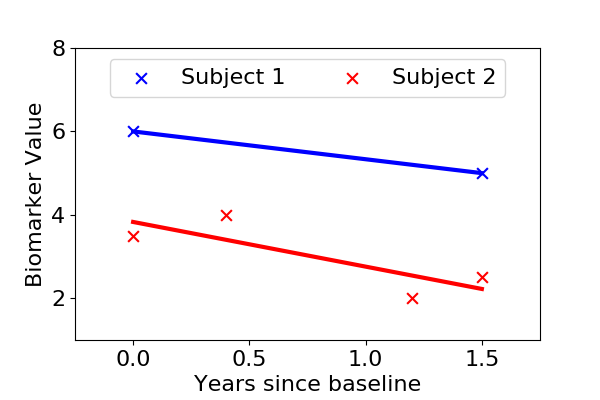
\includegraphics[width=\textwidth]{images/demDiagramPlots/fig1_linReg.png}
    \caption{}
    \label{fig:pcaDemDiagramA}
 \end{subfigure}
 \begin{subfigure}{0.47\textwidth}
     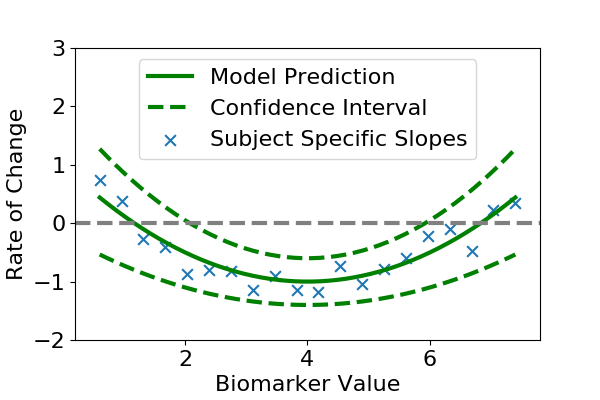
\includegraphics[width=\textwidth]{images/demDiagramPlots/fig2_GP.png}
    \caption{}
    \label{fig:pcaDemDiagramB}
 \end{subfigure}
 \vspace{1em}
 
  \begin{subfigure}{0.47\textwidth}
    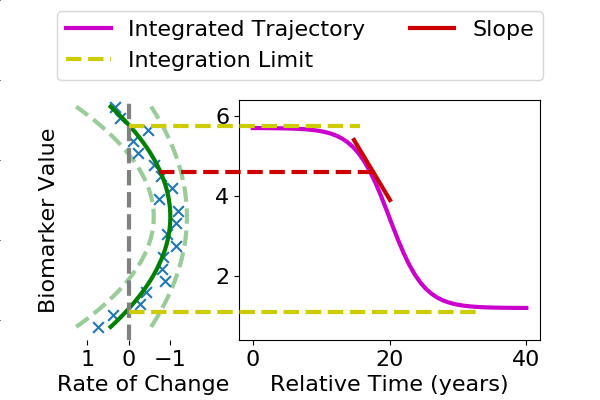
\includegraphics[width=\textwidth]{images/demDiagramPlots/fig3_recon.png}
    \caption{}
    \label{fig:pcaDemDiagramC}
 \end{subfigure}
 \begin{subfigure}{0.47\textwidth}
     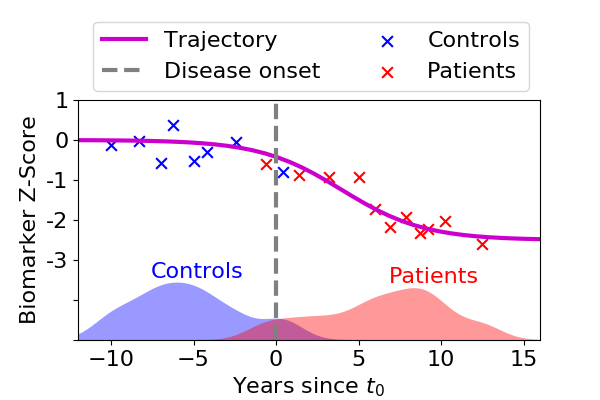
\includegraphics[width=\textwidth]{images/demDiagramPlots/fig4_align.png}
    \caption{}
    \label{fig:pcaDemDiagramD}
 \end{subfigure}
 \caption[Diagram of the Differential Equation Model]{Diagram of the Differential Equation Model. (a) Subject-specific biomarker rates of change were measured from line of best fit, i.e. line slope. (b) Rate of change model: the slopes of each fitted line were plotted against the average biomarker value of each subject (blue crosses). A non-parametric model (Gaussian Process regression, green line) was then fitted on measurements. (c) Trajectory reconstruction: A line integral was performed on the rate of change model. (d) Anchoring process: to give an absolute time reference, the origin $t_0$ was set as the line that best separates controls from patients, which have been staged along the time axis using their biomarker data. Diagram made by me.}
 \label{fig:pcaDemDiagram}
\end{figure}


% DEM
For estimating the rate and extent of biomarker decline, we applied the Differential Equation Model \cite{villemagne2013amyloid, oxtoby2018} (section \ref{sec:bckDem}). The methodology is outlined in Fig. \ref{fig:pcaDemDiagram}. The biomarker measurements for each subject were plotted against time since baseline, and a line was fit for each subject independently. The slope of these lines was then used as a measure of the biomarker rate of change (Fig. \ref{fig:pcaDemDiagramA}). The slopes of each fitted line were then plotted against the average biomarker value of each subject (Fig. \ref{fig:pcaDemDiagramB}). A line integral is then performed on the rate of change model (Fig. \ref{fig:pcaDemDiagramC}).  We repeat the DEM fitting for 8 ROIs independently: the four main lobes, whole brain, ventricles, hippocampus and entorhinal cortex. In order to align all images on a common time frame, we staged the controls and patients based on all their data, and then set an absolute time reference $t_0$ as the line that best separated (i.e. maximised the balanced classification accuracy) the controls' and patients' stages.\footnote{The staging of subjects using all their data required an initial trajectory alignment, which we aligned by initially setting $t_0$ to be the mean biomarker value of patients at baseline.}

There were some adaptations that we performed on the DEM model to ensure a good data fit. In the estimation of the rate of change model (Fig. \ref{fig:pcaDemDiagramB}), we did not include the controls, as there was very little change in their biomarker values. We also normalised the average biomarker values to z-scores and standardised the rates of change by dividing them with the average rate of change of all patients. At the line integration step (Fig. \ref{fig:pcaDemDiagramC}), the integration limits were defined as the biomarker values where the corresponding change is zero or the average biomarker value was equal to the minimum or maximum observed in the dataset. 

After the line integration step, we aligned all trajectories on a common time axis through an anchoring process, where we set the time $t_0 = 0$ to correspond to the value of that biomarker in patients at baseline, averaged across all patients. More precisely, we set $f_j(t_0) = avg(X_j)$ where $f_j$ is the trajectory for biomarker $j$ and $X_j$ are the values of biomarker $j$ in tAD/PCA patients at baseline visit. After this initial anchoring, we staged the subjects along their progression and re-set the $t_0 = 0$ to correspond to the threshold that best separated controls from patients (Fig. \ref{fig:pcaDemDiagramD}). After the anchoring process, we converted all biomarker values to z-scores for comparability (Fig. \ref{fig:pcaDemDiagramD}).

To estimate uncertainty in the trajectories, we sampled 20 trajectories from the posterior distribution of the GP, and then anchored them like the mean trajectory. However, the anchoring would've resulted in zero noise interval at the anchor point, so to get realistic confidence intervals we added to each trajectory an extra amount of random noise $N(0, \sigma)$ on the y-axis, with $\sigma$ set to the standard deviation of the biomarker measurements of each subject at baseline visit.

\subsubsection{Statistical Tests}
% Statistical testing

In order to find out statistically significant differences between the EBM- and DEM-estimated trajectories, we applied several non-parametric statistical tests. 

For EBM results, we tested the effect size of  biomarker $i$ becoming abnormal before another biomarker $j$ both within- and between-group. Within-group differences were assessed using Wilcoxon signed-rank one-tailed tests for all pairs of biomarkers. Between-group (PCA vs tAD) and between-subgroup (space vs object, space vs vision and object vs vision subgroups) differences were assessed using two-tailed Mann-Whitney U tests. We used these non-parametric tests due to non-gaussianity of the data (data is ordinal representing ranks). The reason for using different tests (Wilcoxon vs Mann-Whitney) is because in one case we compare paired samples (two events within the same sequence sample), and in the other unpaired (two events in different sequences, e.g. in a randomly sampled PCA sequence vs a different randomly sampled tAD sequence). We also thinned the MCMC samples (1/100) due to dependence between consecutive samples. 

For DEM results, we tested for differences in estimated biomarker values at different timepoints (-10, 0 and 10 years from $t_0$) both within- and between-groups. For every pair of ROIs, within-group differences were assessed using two-tailed unpaired t-tests. For all ROIs and timepoints, between-group (PCA vs tAD) differences were assessed using similar two-tailed t-tests. For rejecting null hypotheses, we applied Bonferroni-corrected significance thresholds for all tests performed on EBM and DEM results.

\section{Results}
 
% scale parameter for the circles and the gradient
%\tikzset{every picture/.append style={scale=0.5}}
% scale parameter for the upper and lower small brain images
\newcommand*{\scaleBrainImg}{0.25}


\newcommand*{\snapLocationPCA}{\pcaPaperFigs/ebmSnapshotsPCA}
\newcommand*{\snapLocationAD}{\pcaPaperFigs/ebmSnapshotsAD} 
\newcommand*{\snapLocationEAR}{\pcaPaperFigs/ebmSnapshotsEAR} 
\newcommand*{\snapLocationPER}{\pcaPaperFigs/ebmSnapshotsPER} 
\newcommand*{\snapLocationSPA}{\pcaPaperFigs/ebmSnapshotsSPA} 
%col{x}{y}{z} respresents the color for ball z from matrix x at stage y (matrix x, stage y, ball z)

\newcommand*{\snapScale}{0.6} 
\definecolor{light-gray}{gray}{0.6}

\subsection{Progression of PCA and Typical AD}
\label{sec:pcaResPcaAd}

Fig. \ref{fig:pcaSnapshots} shows the maximum likelihood progression of atrophy estimated by the EBM, for both PCA and tAD patients. Snapshots of brain atrophy were taken at model stages 4, 8, 16, 24, 32, 40 and 46 (of 46) using the template from Supplementary Fig. \ref{fig:ebmSnapLabels}. Figure \ref{fig:pcaEBMProg} shows the maximum likelihood sequence and the variance in the main sequence. PCA patients show early atrophy in  occipital areas, ventricles and the superior parietal region, while tAD patients show early atrophy in the amygdala, hippocampus and entorhinal cortex, followed by temporal areas. The ordering is largely preserved under bootstrapping (Supplementary Fig. \ref{fig:bootPosVarAllPcaAd}), and supported by statistical testing (Supplementary Fig. \ref{fig:statTestPcaAd}). Differences in abnormality sequences between PCA and tAD are also statistically significant under Bonferroni corrections (Supplementary Figure \ref{fig:ebmStatTestPcaAd}).
 
Fig. \ref{fig:pcaAdDEM} shows the DEM-estimated biomarker trajectories for PCA (left) and tAD (right). Confidence estimates of the mean trajectory are also given in Fig. \ref{fig:trajDEMPcaAdConf}. Amongst PCA patients, occipital and parietal atrophy was most evident before $t_0$, and by $t_0$ we also observe considerable atrophy in the temporal lobe. Between $t_0$ and 10 years after $t_0$, we observe a marked increase in the rate of occipital, parietal and temporal atrophy and ventricular expansion. By contrast, hippocampal, entorhinal and frontal atrophy never match the extent of tissue loss in posterior and temporal regions. After 10 years from $t_0$, atrophy rates in occipital, parietal and temporal lobes seem to slow down, but limited data in this time window prevents drawing any clear conclusions. Statistical testing within the PCA cohort also confirms our conclusions -- see Supplementary Tables \ref{tab:demStatTestVolsPcaMinus10}, \ref{tab:demStatTestVolsPca0} and \ref{tab:demStatTestVolsPcaPlus10}.

By contrast, before $t_0$ tAD patients showed most extensive tissue loss in the hippocampus, confirmed by significance tests between hippocampal volume and other regions (p $<$ 4e-05, see Supplementary Figs. \ref{tab:demStatTestVolsAdMinus10} and \ref{tab:demStatTestVolsAd0}). After $t_0$, subsequent rates of change are the highest for temporal atrophy and ventricular expansion. It is of note that within 12 years from $t_0$, model estimates of parietal and ventricular abnormality amongst tAD patients are equivalent to or exceed the relative extent of hippocampal abnormality. Comparing PCA and tAD trajectories directly (Fig. \ref{fig:trajDEMPcaAdConf}), the separation between groups at $t_0$ is greatest in parietal (PCA $>$ tAD, p $<$ 1e-6) and hippocampal (tAD $>$ PCA, p $<$ 1e-22) volumes -- see Supplementary table \ref{tab:demStatTestPcaAd} for full statistical testing. 

\subsection{Progression of PCA Subgroups}
\label{sec:pcaResPcaSub}

Fig. \ref{fig:pcaSubgrSnap} shows snapshots of the EBM-estimated atrophy sequence at early stages, in the three cognitively-defined PCA subgroups. The bottom row in the figure shows the uncertainty in the estimated atrophy sequence. The vision subgroup has initial atrophy in the inferior occipital lobe, followed by the angular gyrus, middle temporal, precuneus and superior parietal. The space subgroup shows early atrophy in the superior parietal area (dorsal pattern), followed by inferior occipital and inferior and middle temporal areas. Finally, the object subgroup shows initial atrophy in the middle and inferior occipital areas, with subsequent atrophy in the inferior and middle temporal areas (ventral pattern). Bonferroni-corrected statistically significant differences in atrophy progression have also been observed between PCA subgroups -- see Supplementary Fig. \ref{fig:ebmStatTestPcaSubgroups}. Longitudinal trajectories within PCA subgroups using the DEM could not be estimated due to lack of sufficient data. 


% EBM snapshots
\begin{figure}
  \begin{subfigure}{\textwidth}
   \centering
  % the red-to-yellow gradient on the right
  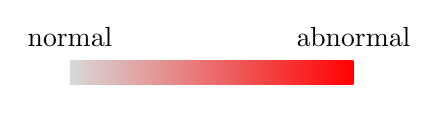
\begin{tikzpicture}[scale=\snapScale,auto,swap]
    \shade[left color=gray!30,right color=red] (0,0) rectangle (6,0.5);
    \node[inner sep=0] (corr_text) at (6,1) {abnormal};
    \node[inner sep=0] (corr_text) at (0,1) {normal};
    \node[inner sep=0] (corr_text) at (0.2,0.5) {};
  \end{tikzpicture}
  \end{subfigure}
  \vspace{1em}
  
    \textbf{\Large{Posterior Cortical Atrophy}}
    
  %\begin{subfigure}[b]{0.15\textwidth}
    \begin{tikzpicture}[scale=\snapScale,auto,swap]

    % the two brain figures on top
    \node (upper_brain) at (0,1.5) { \includegraphics*[scale=\scaleBrainImg,trim=0 0 240 0]{\snapLocationPCA/stage_4.eps}};
    \node (lower_brain) at (0,-1.5) { \includegraphics*[scale=\scaleBrainImg,trim=240 0 0 0]{\snapLocationPCA/stage_4.eps}};
    \node[above=0cm of upper_brain] (stage) {Stage 4};
    % the balls
    
    \end{tikzpicture}
  %\end{subfigure}
  % next subfigure
  \hspace{-1.5em}
  ~
    %\begin{subfigure}[b]{0.15\textwidth}
    \begin{tikzpicture}[scale=\snapScale,auto,swap]

    % the two brain figures on top
    \node (upper_brain) at (0,1.5) { \includegraphics*[scale=\scaleBrainImg,trim=0 0 240 0]{\snapLocationPCA/stage_8.eps}};
    \node (lower_brain) at (0,-1.5) { \includegraphics*[scale=\scaleBrainImg,trim=240 0 0 0]{\snapLocationPCA/stage_8.eps}};
    \node[above=0cm of upper_brain] (stage) {Stage 8};
    % the balls
    
    \end{tikzpicture}
  %\end{subfigure}
  % next subfigure
  \hspace{-1.5em}
  ~
  %\begin{subfigure}[b]{0.15\textwidth}
    \begin{tikzpicture}[scale=\snapScale,auto,swap]

    % the two brain figures on top
    \node (upper_brain) at (0,1.5) { \includegraphics*[scale=\scaleBrainImg,trim=0 0 240 0]{\snapLocationPCA/stage_16.eps}};
    \node (lower_brain) at (0,-1.5) { \includegraphics*[scale=\scaleBrainImg,trim=240 0 0 0]{\snapLocationPCA/stage_16.eps}};
    \node[above=0cm of upper_brain] (stage) {Stage 16};
    % the balls
    
    \end{tikzpicture}
  %\end{subfigure}
  % next subfigure
  \hspace{-1.5em}
  ~
  %\begin{subfigure}[b]{0.15\textwidth}
    \begin{tikzpicture}[scale=\snapScale,auto,swap]

    % the two brain figures on top
    \node (upper_brain) at (0,1.5) { \includegraphics*[scale=\scaleBrainImg,trim=0 0 240 0]{\snapLocationPCA/stage_24.eps}};
    \node (lower_brain) at (0,-1.5) { \includegraphics*[scale=\scaleBrainImg,trim=240 0 0 0]{\snapLocationPCA/stage_24.eps}};
    \node[above=0cm of upper_brain] (stage) {Stage 24};
    % the balls
    
    \end{tikzpicture}
  %\end{subfigure}
  % next subfigure
  \hspace{-1.5em}
  ~
  %\begin{subfigure}[b]{0.15\textwidth}
    \begin{tikzpicture}[scale=\snapScale,auto,swap]

    % the two brain figures on top
    \node (upper_brain) at (0,1.5) { \includegraphics*[scale=\scaleBrainImg,trim=0 0 240 0]{\snapLocationPCA/stage_32.eps}};
    \node (lower_brain) at (0,-1.5) { \includegraphics*[scale=\scaleBrainImg,trim=240 0 0 0]{\snapLocationPCA/stage_32.eps}};
    \node[above=0cm of upper_brain] (stage) {Stage 32};
    % the balls
    
    \end{tikzpicture}
  %\end{subfigure}
  % next subfigure
  \hspace{-1.5em}
  ~
  %\begin{subfigure}[b]{0.15\textwidth}
    \begin{tikzpicture}[scale=\snapScale,auto,swap]

    % the two brain figures on top
    \node (upper_brain) at (0,1.5) { \includegraphics*[scale=\scaleBrainImg,trim=0 0 240 0]{\snapLocationPCA/stage_40.eps}};
    \node (lower_brain) at (0,-1.5) { \includegraphics*[scale=\scaleBrainImg,trim=240 0 0 0]{\snapLocationPCA/stage_40.eps}};
    \node[above=0cm of upper_brain] (stage) {Stage 40};
    % the balls
    
    \end{tikzpicture}
  %\end{subfigure}
  % next subfigure
  \hspace{-1.5em}
  ~
  %\begin{subfigure}[b]{0.15\textwidth}
    \begin{tikzpicture}[scale=\snapScale,auto,swap]

    % the two brain figures on top
    \node (upper_brain) at (0,1.5) { \includegraphics*[scale=\scaleBrainImg,trim=0 0 240 0]{\snapLocationPCA/stage_46.eps}};
    \node (lower_brain) at (0,-1.5) { \includegraphics*[scale=\scaleBrainImg,trim=240 0 0 0]{\snapLocationPCA/stage_46.eps}};
    \node[above=0cm of upper_brain] (stage) {Stage 46};
    % the balls
    
    \end{tikzpicture}
  %\end{subfigure}
  % next subfigure
  \hspace{-1.5em}
  
  \textbf{\Large{Typical Alzheimer's Disease}}

%   \centering
  %\begin{subfigure}[b]{0.15\textwidth}
    \begin{tikzpicture}[scale=\snapScale,auto,swap]

    % the two brain figures on top
    \node (upper_brain) at (0,1.5) { \includegraphics*[scale=\scaleBrainImg,trim=0 0 240 0]{\snapLocationAD/stage_4.eps}};
    \node (lower_brain) at (0,-1.5) { \includegraphics*[scale=\scaleBrainImg,trim=240 0 0 0]{\snapLocationAD/stage_4.eps}};
    \node[above=0cm of upper_brain] (stage) {Stage 4};
    % the balls
    
    \end{tikzpicture}
  %\end{subfigure}
  % next subfigure
  \hspace{-1.5em}
  ~
    %\begin{subfigure}[b]{0.15\textwidth}
    \begin{tikzpicture}[scale=\snapScale,auto,swap]

    % the two brain figures on top
    \node (upper_brain) at (0,1.5) { \includegraphics*[scale=\scaleBrainImg,trim=0 0 240 0]{\snapLocationAD/stage_8.eps}};
    \node (lower_brain) at (0,-1.5) { \includegraphics*[scale=\scaleBrainImg,trim=240 0 0 0]{\snapLocationAD/stage_8.eps}};
    \node[above=0cm of upper_brain] (stage) {Stage 8};
    % the balls
    
    \end{tikzpicture}
  %\end{subfigure}
  % next subfigure
  \hspace{-1.5em}
  ~
  %\begin{subfigure}[b]{0.15\textwidth}
    \begin{tikzpicture}[scale=\snapScale,auto,swap]

    % the two brain figures on top
    \node (upper_brain) at (0,1.5) { \includegraphics*[scale=\scaleBrainImg,trim=0 0 240 0]{\snapLocationAD/stage_16.eps}};
    \node (lower_brain) at (0,-1.5) { \includegraphics*[scale=\scaleBrainImg,trim=240 0 0 0]{\snapLocationAD/stage_16.eps}};
    \node[above=0cm of upper_brain] (stage) {Stage 16};
    % the balls
    
    \end{tikzpicture}
  %\end{subfigure}
  % next subfigure
  \hspace{-1.5em}
  ~
  %\begin{subfigure}[b]{0.15\textwidth}
    \begin{tikzpicture}[scale=\snapScale,auto,swap]

    % the two brain figures on top
    \node (upper_brain) at (0,1.5) { \includegraphics*[scale=\scaleBrainImg,trim=0 0 240 0]{\snapLocationAD/stage_24.eps}};
    \node (lower_brain) at (0,-1.5) { \includegraphics*[scale=\scaleBrainImg,trim=240 0 0 0]{\snapLocationAD/stage_24.eps}};
    \node[above=0cm of upper_brain] (stage) {Stage 24};
    % the balls
    
    \end{tikzpicture}
  %\end{subfigure}
  % next subfigure
  \hspace{-1.5em}
  ~
  %\begin{subfigure}[b]{0.15\textwidth}
    \begin{tikzpicture}[scale=\snapScale,auto,swap]

    % the two brain figures on top
    \node (upper_brain) at (0,1.5) { \includegraphics*[scale=\scaleBrainImg,trim=0 0 240 0]{\snapLocationAD/stage_32.eps}};
    \node (lower_brain) at (0,-1.5) { \includegraphics*[scale=\scaleBrainImg,trim=240 0 0 0]{\snapLocationAD/stage_32.eps}};
    \node[above=0cm of upper_brain] (stage) {Stage 32};
    % the balls
    
    \end{tikzpicture}
  %\end{subfigure}
  % next subfigure
  \hspace{-1.5em}
  ~
  %\begin{subfigure}[b]{0.15\textwidth}
    \begin{tikzpicture}[scale=\snapScale,auto,swap]

    % the two brain figures on top
    \node (upper_brain) at (0,1.5) { \includegraphics*[scale=\scaleBrainImg,trim=0 0 240 0]{\snapLocationAD/stage_40.eps}};
    \node (lower_brain) at (0,-1.5) { \includegraphics*[scale=\scaleBrainImg,trim=240 0 0 0]{\snapLocationAD/stage_40.eps}};
    \node[above=0cm of upper_brain] (stage) {Stage 40};
    % the balls
    
    \end{tikzpicture}
  %\end{subfigure}
  % next subfigure
  \hspace{-1.5em}
  ~
  %\begin{subfigure}[b]{0.15\textwidth}
    \begin{tikzpicture}[scale=\snapScale,auto,swap]

    % the two brain figures on top
    \node (upper_brain) at (0,1.5) { \includegraphics*[scale=\scaleBrainImg,trim=0 0 240 0]{\snapLocationAD/stage_46.eps}};
    \node (lower_brain) at (0,-1.5) { \includegraphics*[scale=\scaleBrainImg,trim=240 0 0 0]{\snapLocationAD/stage_46.eps}};
    \node[above=0cm of upper_brain] (stage) {Stage 46};
    % the balls
    
    \end{tikzpicture}
  %\end{subfigure}
  % next subfigure
  \hspace{-1.5em}
  
\caption[Atrophy progression in PCA and tAD patients according to the event-based model]{Atrophy progression in PCA and tAD patients according to the event-based model. White regions are within the volume range of healthy controls, while red regions show abnormally low volumes by the corresponding stage, with shading indicating the probability of abnormality. By each stage, a number of biomarkers shaded in red became abnormal. Brain pictures generated using BrainPainter \cite{marinescu2019BrainPainter}}  
\label{fig:pcaSnapshots}
\end{figure}

% EBM positional variance matrices
\begin{figure}
\centering
  \begin{subfigure}{0.7\textwidth}
  \centering
 \textbf{\large{\mbox{Posterior Cortical Atrophy}}}
 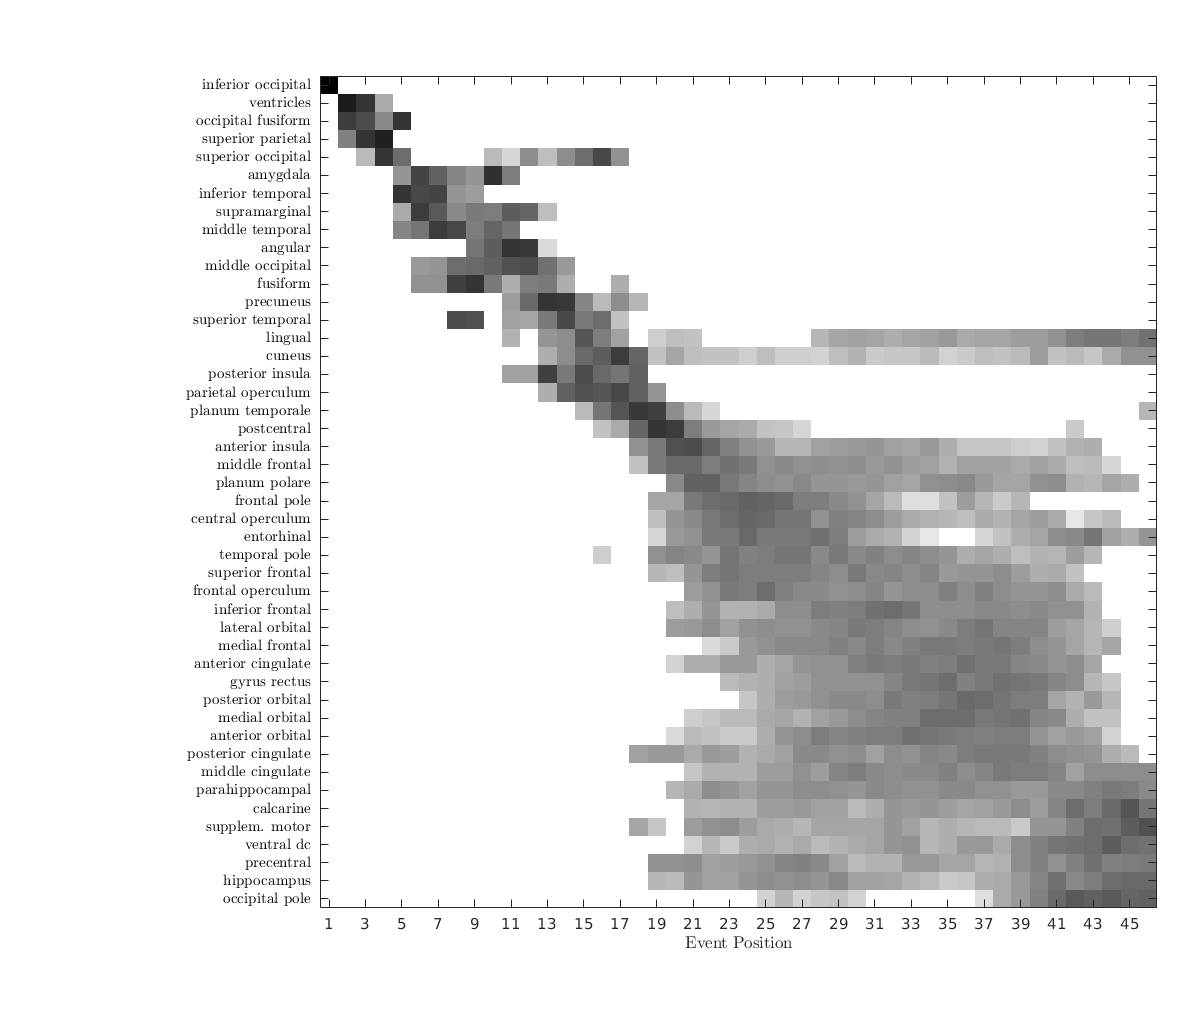
\includegraphics[width=1\textwidth,trim=100 30 0 50,clip]{\pcaPaperFigs/posVarianceMatrixPCA.png} 
 \end{subfigure}
 \hspace{1em}
  \begin{subfigure}{0.7\textwidth}
  \centering
  \textbf{\large{\mbox{Typical Alzheimer's Disease}}}
 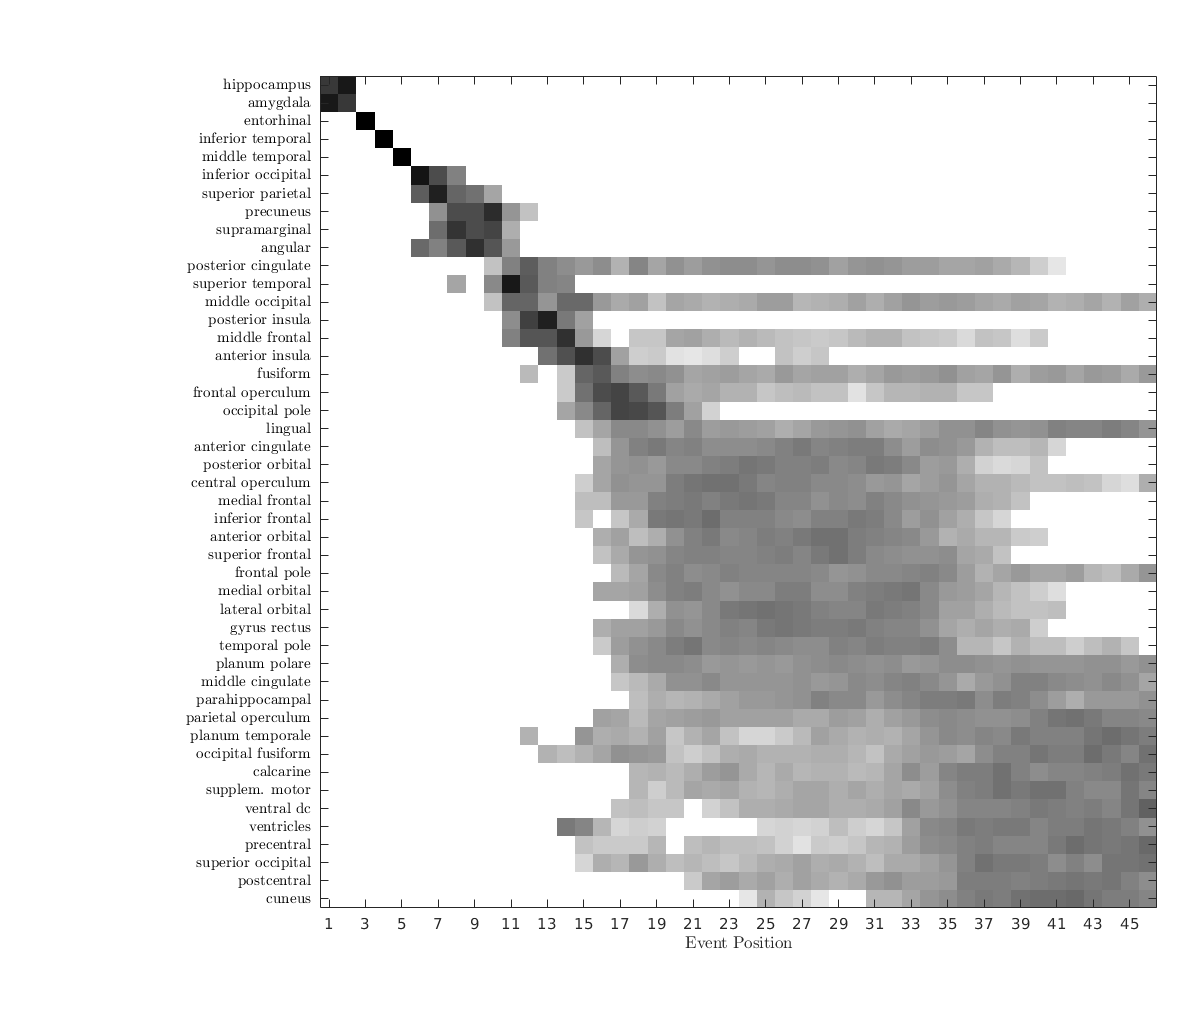
\includegraphics[width=1\textwidth,trim=100 30 0 50,clip]{\pcaPaperFigs/posVarianceMatrixAD.png}
%  \caption{}
 \end{subfigure}
 \caption[PCA and tAD positional variance diagrams estimated by the EBM]{Uncertainty in the EBM-estimated atrophy sequences for (top) PCA and (bottom) tAD from Fig \ref{fig:pcaSnapshots}. The ROIs on the Y-axis are ordered according to the timing of abnormality, from early abnormalities on the top to late abnormalities on the bottom. The X-axis shows the position of a biomarker in the abnormality sequence. Each pixel at position $(i,j)$ shows the probability of biomarker $j$ becoming abnormal at position $i$, with darker squares showing higher confidence and whiter squares showing lower confidence. The biomarker orderings are sampled from the EBM posterior distribution.}
 \label{fig:pcaEBMProg}
\end{figure}

% DEM average traj
\begin{figure}
 \centering
\begin{subfigure}{0.8\textwidth}
 \centering
 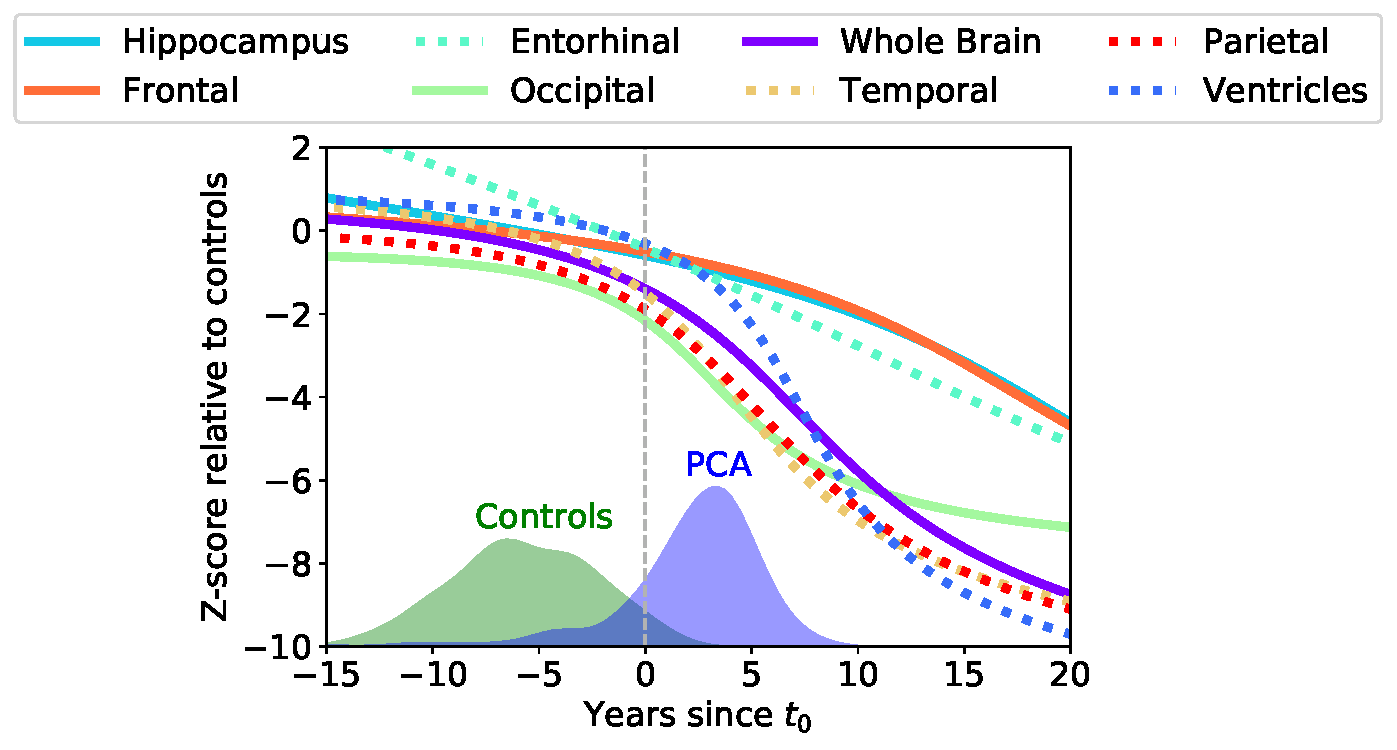
\includegraphics[width=0.8\textwidth,trim=0 300 0 0,clip]{\pcaPaperFigs/trajAlign_600_500PCA.pdf}
\end{subfigure}
 
 \begin{subfigure}{0.47\textwidth}
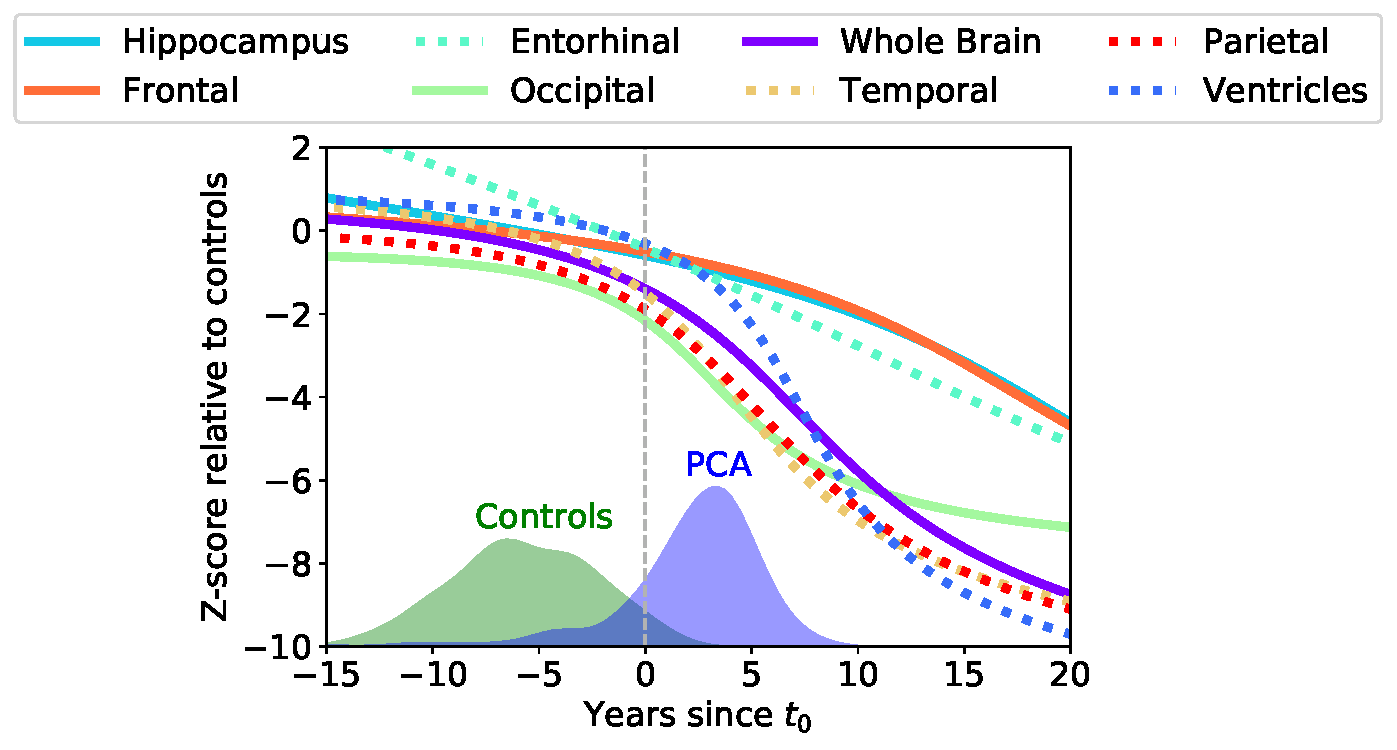
\includegraphics[width=\textwidth,trim=90 0 120 60,clip]{\pcaPaperFigs/trajAlign_600_500PCA.pdf}
 \caption{PCA}
 \label{trajDEMPCA} 
 \end{subfigure}
 \begin{subfigure}{0.47\textwidth}
 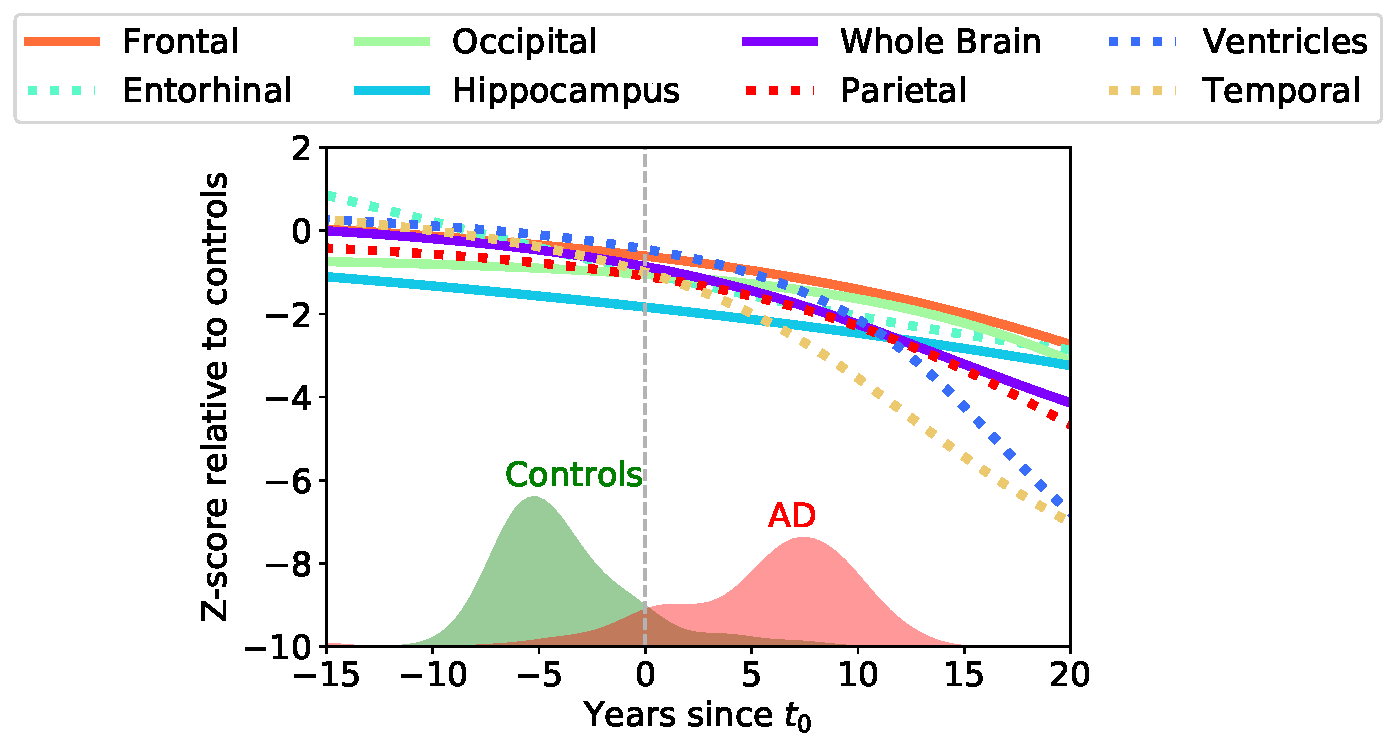
\includegraphics[width=\textwidth,trim=90 0 120 60,clip]{\pcaPaperFigs/trajAlign_600_500AD.pdf}
 \caption{tAD}
 \label{trajDEMAD}
 \end{subfigure}
 \caption[PCA and tAD trajectories estimated by the DEM]{(a-b) Trajectories of different ROI volumes from the differential equation model for (a) PCA progression and (b) tAD progression. The x-axis shows the number of years since $t_0$, and the y-axis shows the z-score of the ROI volume relative to controls. The trajectories of the ventricles have been flipped to aid comparison. Overlayed are histograms of subject stages based on the estimated trajectories.}
 \label{fig:pcaAdDEM}
\end{figure}

% DEM confidence estimates
\begin{figure}
 \centering
 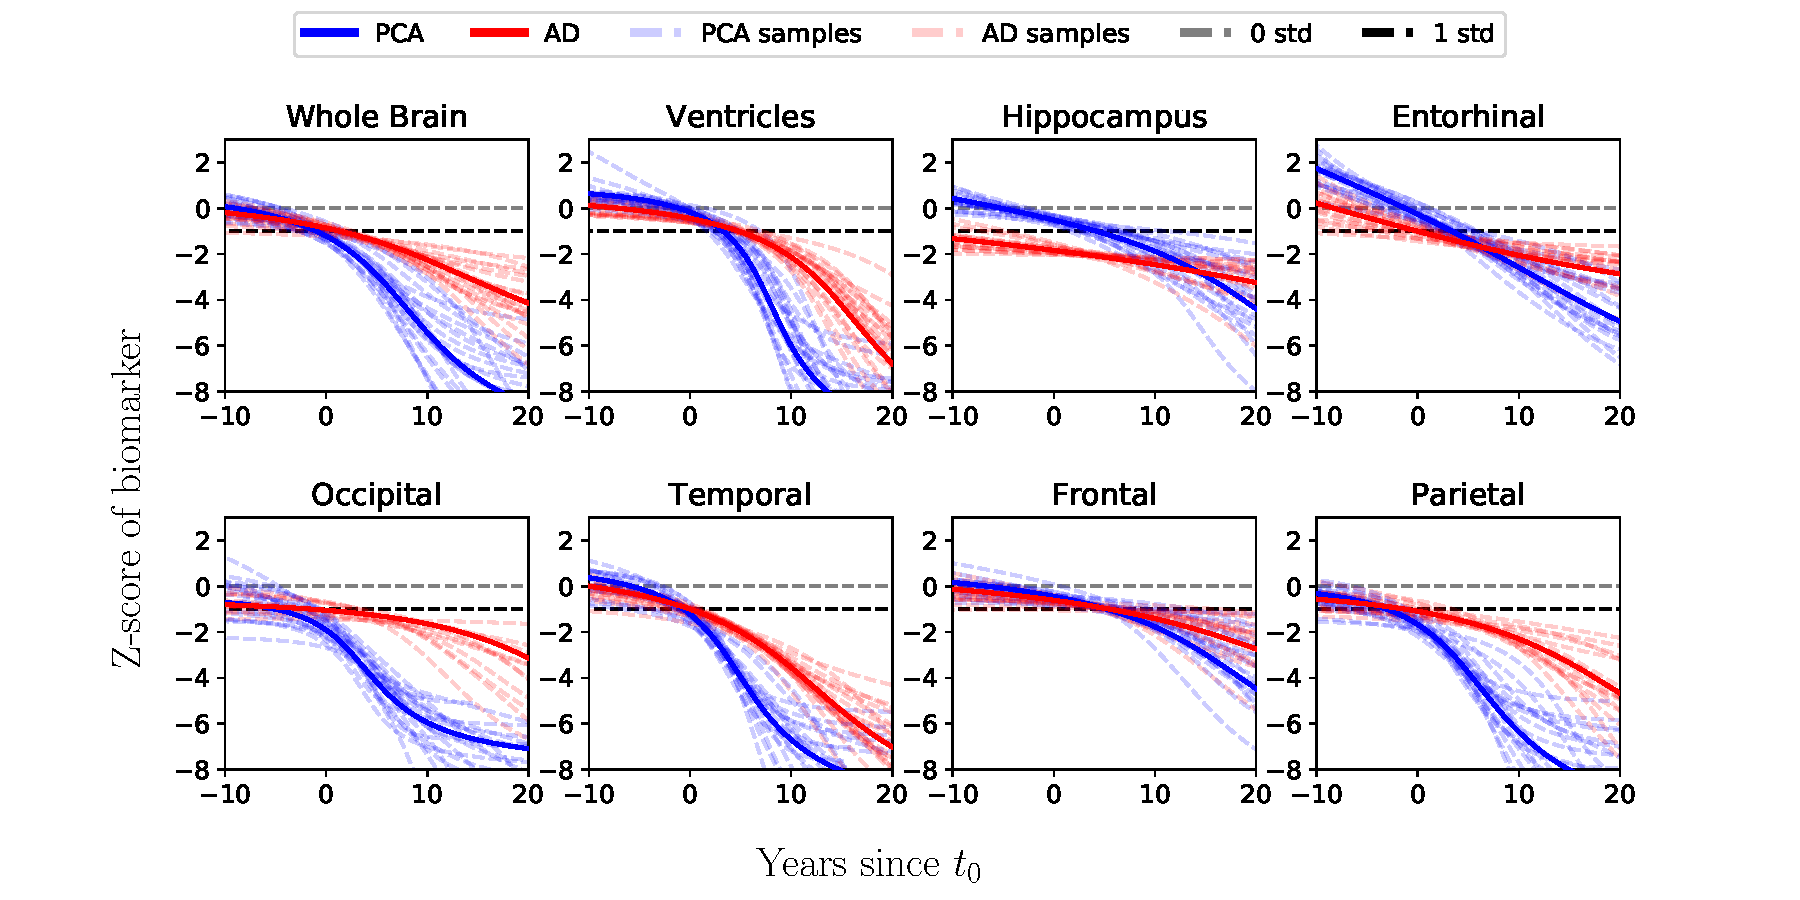
\includegraphics[width=\textwidth, trim=50 0 50 0]{\pcaPaperFigs/subplotsPcaAd.pdf}
 \caption[PCA and tAD trajectories aligned in the same space, with samples from the posterior distribution]{Mean trajectories for ROI volumes for PCA and tAD aligned on the same temporal scale with samples from the posterior distribution showing the confidence of the mean trajectory. The axis shows the number of years since $t_0$, and the y-axis shows the z-score of the ROI volume relative to controls. The trajectories for the ventricles have been flipped to aid visual comparison. The 1 std and 0 std horizontal lines represent the limit of 1 and 0 standard deviations away from the mean values of controls.}
 \label{fig:trajDEMPcaAdConf}
\end{figure}

% subgroup EBM results
\begin{figure}
  \begin{subfigure}{\textwidth}
   \centering
  % the red-to-yellow gradient on the right
  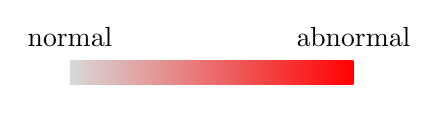
\begin{tikzpicture}[scale=\snapScale,auto,swap]
    \shade[left color=gray!30,right color=red] (0,0) rectangle (6,0.5);
    \node[inner sep=0] (corr_text) at (6,1) {abnormal};
    \node[inner sep=0] (corr_text) at (0,1) {normal};
    \node[inner sep=0] (corr_text) at (0.2,0.5) {};
  \end{tikzpicture}
  \end{subfigure}
%   \vspace{1em}

%   \centering
  {\Large \textbf{Vision impairment group}\par}
  %\begin{subfigure}[b]{0.15\textwidth}
    \begin{tikzpicture}[scale=\snapScale,auto,swap]

    % the two brain figures on top
    \node (upper_brain) at (0,1.5) { \includegraphics*[scale=\scaleBrainImg,trim=0 0 240 0]{\snapLocationEAR/stage_1.eps}};
    \node (lower_brain) at (0,-1.5) { \includegraphics*[scale=\scaleBrainImg,trim=240 0 0 0]{\snapLocationEAR/stage_1.eps}};
    \node[above=0cm of upper_brain] (stage) {Stage 1};
    % the balls
    
    \end{tikzpicture}
  %\end{subfigure}
  % next subfigure
  \hspace{-1.5em}
  ~
  %\begin{subfigure}[b]{0.15\textwidth}
    \begin{tikzpicture}[scale=\snapScale,auto,swap]

    % the two brain figures on top
    \node (upper_brain) at (0,1.5) { \includegraphics*[scale=\scaleBrainImg,trim=0 0 240 0]{\snapLocationEAR/stage_2.eps}};
    \node (lower_brain) at (0,-1.5) { \includegraphics*[scale=\scaleBrainImg,trim=240 0 0 0]{\snapLocationEAR/stage_2.eps}};
    \node[above=0cm of upper_brain] (stage) {Stage 2};
    % the balls
    
    \end{tikzpicture}
  %\end{subfigure}
  % next subfigure
  \hspace{-1.5em}
  ~
  %\begin{subfigure}[b]{0.15\textwidth}
    \begin{tikzpicture}[scale=\snapScale,auto,swap]

    % the two brain figures on top
    \node (upper_brain) at (0,1.5) { \includegraphics*[scale=\scaleBrainImg,trim=0 0 240 0]{\snapLocationEAR/stage_3.eps}};
    \node (lower_brain) at (0,-1.5) { \includegraphics*[scale=\scaleBrainImg,trim=240 0 0 0]{\snapLocationEAR/stage_3.eps}};
    \node[above=0cm of upper_brain] (stage) {Stage 3};
    % the balls
    
    \end{tikzpicture}
  %\end{subfigure}
  % next subfigure
  \hspace{-1.5em}
  ~
  %\begin{subfigure}[b]{0.15\textwidth}
    \begin{tikzpicture}[scale=\snapScale,auto,swap]

    % the two brain figures on top
    \node (upper_brain) at (0,1.5) { \includegraphics*[scale=\scaleBrainImg,trim=0 0 240 0]{\snapLocationEAR/stage_4.eps}};
    \node (lower_brain) at (0,-1.5) { \includegraphics*[scale=\scaleBrainImg,trim=240 0 0 0]{\snapLocationEAR/stage_4.eps}};
    \node[above=0cm of upper_brain] (stage) {Stage 4};
    % the balls
    
    \end{tikzpicture}
  %\end{subfigure}
  % next subfigure
  \hspace{-1.5em}
  ~
  %\begin{subfigure}[b]{0.15\textwidth}
    \begin{tikzpicture}[scale=\snapScale,auto,swap]

    % the two brain figures on top
    \node (upper_brain) at (0,1.5) { \includegraphics*[scale=\scaleBrainImg,trim=0 0 240 0]{\snapLocationEAR/stage_5.eps}};
    \node (lower_brain) at (0,-1.5) { \includegraphics*[scale=\scaleBrainImg,trim=240 0 0 0]{\snapLocationEAR/stage_5.eps}};
    \node[above=0cm of upper_brain] (stage) {Stage 5};
    % the balls
    
    \end{tikzpicture}
  %\end{subfigure}
  % next subfigure
  \hspace{-1.5em}
  ~
  %\begin{subfigure}[b]{0.15\textwidth}
    \begin{tikzpicture}[scale=\snapScale,auto,swap]

    % the two brain figures on top
    \node (upper_brain) at (0,1.5) { \includegraphics*[scale=\scaleBrainImg,trim=0 0 240 0]{\snapLocationEAR/stage_6.eps}};
    \node (lower_brain) at (0,-1.5) { \includegraphics*[scale=\scaleBrainImg,trim=240 0 0 0]{\snapLocationEAR/stage_6.eps}};
    \node[above=0cm of upper_brain] (stage) {Stage 6};
    % the balls
    
    \end{tikzpicture}
  %\end{subfigure}
  % next subfigure
  \hspace{-1.5em}
  ~
  %\begin{subfigure}[b]{0.15\textwidth}
    \begin{tikzpicture}[scale=\snapScale,auto,swap]

    % the two brain figures on top
    \node (upper_brain) at (0,1.5) { \includegraphics*[scale=\scaleBrainImg,trim=0 0 240 0]{\snapLocationEAR/stage_7.eps}};
    \node (lower_brain) at (0,-1.5) { \includegraphics*[scale=\scaleBrainImg,trim=240 0 0 0]{\snapLocationEAR/stage_7.eps}};
    \node[above=0cm of upper_brain] (stage) {Stage 7};
    % the balls
    
    \end{tikzpicture}

    \hspace{-1.5em}


    \vspace{-1em}

    {\Large \textbf{Space perception impairment group}\par}
    \begin{tikzpicture}[scale=\snapScale,auto,swap]

    % the two brain figures on top
    \node (upper_brain) at (0,1.5) { \includegraphics*[scale=\scaleBrainImg,trim=0 0 240 0]{\snapLocationSPA/stage_1.eps}};
    \node (lower_brain) at (0,-1.5) { \includegraphics*[scale=\scaleBrainImg,trim=240 0 0 0]{\snapLocationSPA/stage_1.eps}};
    \node[above=0cm of upper_brain] (stage) {Stage 1};
    % the balls
    
    \end{tikzpicture}
  %\end{subfigure}
  % next subfigure
  \hspace{-1.5em}
  ~
  %\begin{subfigure}[b]{0.15\textwidth}
    \begin{tikzpicture}[scale=\snapScale,auto,swap]

    % the two brain figures on top
    \node (upper_brain) at (0,1.5) { \includegraphics*[scale=\scaleBrainImg,trim=0 0 240 0]{\snapLocationSPA/stage_2.eps}};
    \node (lower_brain) at (0,-1.5) { \includegraphics*[scale=\scaleBrainImg,trim=240 0 0 0]{\snapLocationSPA/stage_2.eps}};
    \node[above=0cm of upper_brain] (stage) {Stage 2};
    % the balls
    
    \end{tikzpicture}
  %\end{subfigure}
  % next subfigure
  \hspace{-1.5em}
  ~
  %\begin{subfigure}[b]{0.15\textwidth}
    \begin{tikzpicture}[scale=\snapScale,auto,swap]

    % the two brain figures on top
    \node (upper_brain) at (0,1.5) { \includegraphics*[scale=\scaleBrainImg,trim=0 0 240 0]{\snapLocationSPA/stage_3.eps}};
    \node (lower_brain) at (0,-1.5) { \includegraphics*[scale=\scaleBrainImg,trim=240 0 0 0]{\snapLocationSPA/stage_3.eps}};
    \node[above=0cm of upper_brain] (stage) {Stage 3};
    % the balls
    
    \end{tikzpicture}
  %\end{subfigure}
  % next subfigure
  \hspace{-1.5em}
  ~
  %\begin{subfigure}[b]{0.15\textwidth}
    \begin{tikzpicture}[scale=\snapScale,auto,swap]

    % the two brain figures on top
    \node (upper_brain) at (0,1.5) { \includegraphics*[scale=\scaleBrainImg,trim=0 0 240 0]{\snapLocationSPA/stage_4.eps}};
    \node (lower_brain) at (0,-1.5) { \includegraphics*[scale=\scaleBrainImg,trim=240 0 0 0]{\snapLocationSPA/stage_4.eps}};
    \node[above=0cm of upper_brain] (stage) {Stage 4};
    % the balls
    
    \end{tikzpicture}
  %\end{subfigure}
  % next subfigure
  \hspace{-1.5em}
  ~
  %\begin{subfigure}[b]{0.15\textwidth}
    \begin{tikzpicture}[scale=\snapScale,auto,swap]

    % the two brain figures on top
    \node (upper_brain) at (0,1.5) { \includegraphics*[scale=\scaleBrainImg,trim=0 0 240 0]{\snapLocationSPA/stage_5.eps}};
    \node (lower_brain) at (0,-1.5) { \includegraphics*[scale=\scaleBrainImg,trim=240 0 0 0]{\snapLocationSPA/stage_5.eps}};
    \node[above=0cm of upper_brain] (stage) {Stage 5};
    % the balls
    
    \end{tikzpicture}
  %\end{subfigure}
  % next subfigure
  \hspace{-1.5em}
  ~
  %\begin{subfigure}[b]{0.15\textwidth}
    \begin{tikzpicture}[scale=\snapScale,auto,swap]

    % the two brain figures on top
    \node (upper_brain) at (0,1.5) { \includegraphics*[scale=\scaleBrainImg,trim=0 0 240 0]{\snapLocationSPA/stage_6.eps}};
    \node (lower_brain) at (0,-1.5) { \includegraphics*[scale=\scaleBrainImg,trim=240 0 0 0]{\snapLocationSPA/stage_6.eps}};
    \node[above=0cm of upper_brain] (stage) {Stage 6};
    % the balls
    
    \end{tikzpicture}
  %\end{subfigure}
  % next subfigure
  \hspace{-1.5em}
  ~
  %\begin{subfigure}[b]{0.15\textwidth}
    \begin{tikzpicture}[scale=\snapScale,auto,swap]

    % the two brain figures on top
    \node (upper_brain) at (0,1.5) { \includegraphics*[scale=\scaleBrainImg,trim=0 0 240 0]{\snapLocationSPA/stage_7.eps}};
    \node (lower_brain) at (0,-1.5) { \includegraphics*[scale=\scaleBrainImg,trim=240 0 0 0]{\snapLocationSPA/stage_7.eps}};
    \node[above=0cm of upper_brain] (stage) {Stage 7};
    % the balls
    
    \end{tikzpicture}
  %\end{subfigure}
  % next subfigure
  \hspace{-1.5em}


\vspace{-1em}


%   \centering
  %\begin{subfigure}[b]{0.15\textwidth}
    {\Large \textbf{Object perception impairment group}\par}
    \begin{tikzpicture}[scale=\snapScale,auto,swap]

    % the two brain figures on top
    \node (upper_brain) at (0,1.5) { \includegraphics*[scale=\scaleBrainImg,trim=0 0 240 0]{\snapLocationPER/stage_1.eps}};
    \node (lower_brain) at (0,-1.5) { \includegraphics*[scale=\scaleBrainImg,trim=240 0 0 0]{\snapLocationPER/stage_1.eps}};
    \node[above=0cm of upper_brain] (stage) {Stage 1};
    % the balls
    
    \end{tikzpicture}
  %\end{subfigure}
  % next subfigure
  \hspace{-1.5em}
  ~
  %\begin{subfigure}[b]{0.15\textwidth}
    \begin{tikzpicture}[scale=\snapScale,auto,swap]

    % the two brain figures on top
    \node (upper_brain) at (0,1.5) { \includegraphics*[scale=\scaleBrainImg,trim=0 0 240 0]{\snapLocationPER/stage_2.eps}};
    \node (lower_brain) at (0,-1.5) { \includegraphics*[scale=\scaleBrainImg,trim=240 0 0 0]{\snapLocationPER/stage_2.eps}};
    \node[above=0cm of upper_brain] (stage) {Stage 2};
    % the balls
    
    \end{tikzpicture}
  %\end{subfigure}
  % next subfigure
  \hspace{-1.5em}
  ~
  %\begin{subfigure}[b]{0.15\textwidth}
    \begin{tikzpicture}[scale=\snapScale,auto,swap]

    % the two brain figures on top
    \node (upper_brain) at (0,1.5) { \includegraphics*[scale=\scaleBrainImg,trim=0 0 240 0]{\snapLocationPER/stage_3.eps}};
    \node (lower_brain) at (0,-1.5) { \includegraphics*[scale=\scaleBrainImg,trim=240 0 0 0]{\snapLocationPER/stage_3.eps}};
    \node[above=0cm of upper_brain] (stage) {Stage 3};
    % the balls
    
    \end{tikzpicture}
  %\end{subfigure}
  % next subfigure
  \hspace{-1.5em}
  ~
  %\begin{subfigure}[b]{0.15\textwidth}
    \begin{tikzpicture}[scale=\snapScale,auto,swap]

    % the two brain figures on top
    \node (upper_brain) at (0,1.5) { \includegraphics*[scale=\scaleBrainImg,trim=0 0 240 0]{\snapLocationPER/stage_4.eps}};
    \node (lower_brain) at (0,-1.5) { \includegraphics*[scale=\scaleBrainImg,trim=240 0 0 0]{\snapLocationPER/stage_4.eps}};
    \node[above=0cm of upper_brain] (stage) {Stage 4};
    % the balls
    
    \end{tikzpicture}
  %\end{subfigure}
  % next subfigure
  \hspace{-1.5em}
  ~
  %\begin{subfigure}[b]{0.15\textwidth}
    \begin{tikzpicture}[scale=\snapScale,auto,swap]

    % the two brain figures on top
    \node (upper_brain) at (0,1.5) { \includegraphics*[scale=\scaleBrainImg,trim=0 0 240 0]{\snapLocationPER/stage_5.eps}};
    \node (lower_brain) at (0,-1.5) { \includegraphics*[scale=\scaleBrainImg,trim=240 0 0 0]{\snapLocationPER/stage_5.eps}};
    \node[above=0cm of upper_brain] (stage) {Stage 5};
    % the balls
    
    \end{tikzpicture}
  %\end{subfigure}
  % next subfigure
  \hspace{-1.5em}
  ~
  %\begin{subfigure}[b]{0.15\textwidth}
    \begin{tikzpicture}[scale=\snapScale,auto,swap]

    % the two brain figures on top
    \node (upper_brain) at (0,1.5) { \includegraphics*[scale=\scaleBrainImg,trim=0 0 240 0]{\snapLocationPER/stage_6.eps}};
    \node (lower_brain) at (0,-1.5) { \includegraphics*[scale=\scaleBrainImg,trim=240 0 0 0]{\snapLocationPER/stage_6.eps}};
    \node[above=0cm of upper_brain] (stage) {Stage 6};
    % the balls
    
    \end{tikzpicture}
  %\end{subfigure}
  % next subfigure
  \hspace{-1.5em}
  ~
  %\begin{subfigure}[b]{0.15\textwidth}
    \begin{tikzpicture}[scale=\snapScale,auto,swap]

    % the two brain figures on top
    \node (upper_brain) at (0,1.5) { \includegraphics*[scale=\scaleBrainImg,trim=0 0 240 0]{\snapLocationPER/stage_7.eps}};
    \node (lower_brain) at (0,-1.5) { \includegraphics*[scale=\scaleBrainImg,trim=240 0 0 0]{\snapLocationPER/stage_7.eps}};
    \node[above=0cm of upper_brain] (stage) {Stage 7};
    % the balls
    
    \end{tikzpicture}
  %\end{subfigure}
  % next subfigure
  \hspace{-1.5em}

  
 \begin{subfigure}{0.32\textwidth}
 \centering
 {\footnotesize \textbf{Vision}\par}
 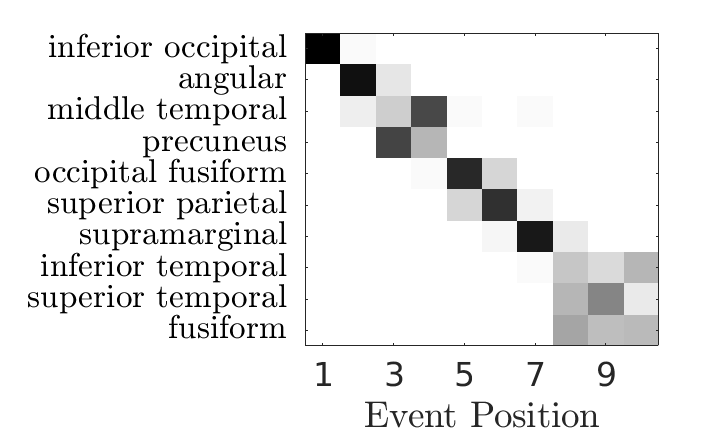
\includegraphics[width=\textwidth]{\pcaPaperFigs/posVarianceMatSmall10EAR.png}
 \end{subfigure}
  \begin{subfigure}{0.32\textwidth}
  \centering
  {\footnotesize \textbf{Space}\par}
 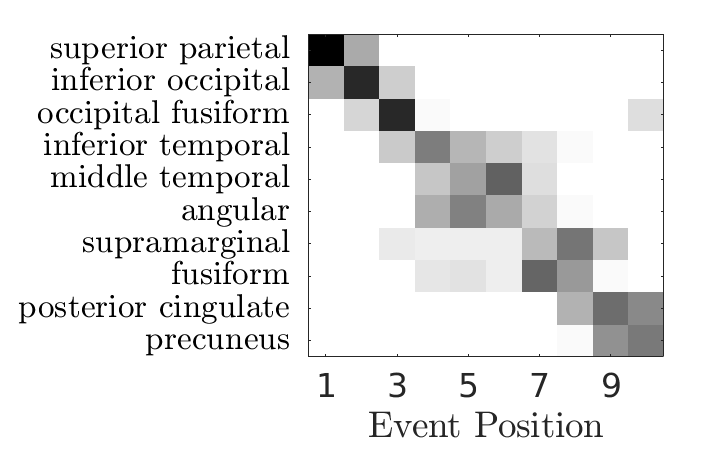
\includegraphics[width=\textwidth]{\pcaPaperFigs/posVarianceMatSmall10SPA.png}
 \end{subfigure}
  \begin{subfigure}{0.32\textwidth}
  \centering
  {\footnotesize \textbf{Object}\par}
 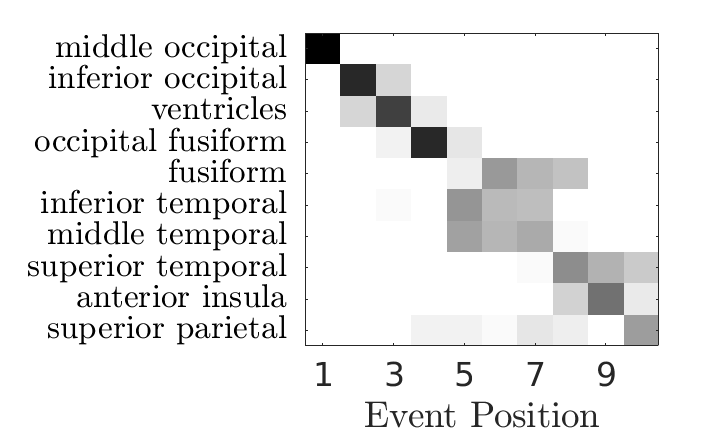
\includegraphics[width=\textwidth]{\pcaPaperFigs/posVarianceMatSmall10PER.png}
 \end{subfigure}
 \caption[Early atrophy progression within the three cognitively-defined PCA subgroups]{Early atrophy progression within the three cognitively-defined PCA subgroups, as estimated by the EBM. The top figures shows snapshots of the atrophy patterns for the first 7 stages in the EBM, while the last row shows the uncertainty in the atrophy progression sequence. Brain pictures generated using BrainPainter \cite{marinescu2019BrainPainter}}
 \label{fig:pcaSubgrSnap}
\end{figure}

\section{Discussion}
\label{sec:pcaDis}

% summary of findings
In this work we performed one of the first longitudinal studies of atrophy progression in PCA. Results suggest that in PCA occipital and superior parietal areas are the first to become affected, followed by temporal areas. By 10 years after $t_0$, there seems to be widespread atrophy in the occipital, parietal and temporal areas, as well as ventricular expansion. In contrast, tAD seems to have significant early atrophy in the hippocampus, with subsequent temporal atrophy and ventricular expansion starting 5 years after $t_0$. 

% talk about heterogeneity 
Regarding PCA heterogeneity, our study also provided the first glimpse into the early longitudinal patterns of atrophy within three cognitively defined PCA subtypes. We found early phenotype-specific patterns of atrophy within each cognitively-defined PCA subgroup. These patterns of pathology overlap with the pathways that are hypothesised to be affected within each group: striate cortex for the vision subgroup, dorsal pathway for the space subgroup and ventral pathway for the object subgroup. Nonetheless, among the subgroups there is considerable variability in these patterns as well as spatial overlap, which might suggest that these should not necessarily be interpreted as distinct diseases, but rather that the patients lie on a continuum of phenotypical variation, as suggested by \cite{lehmann2011basic}. 

% Strengths of the EBM and DEM methodology 
Our study has several strengths. First of all, the large number of PCA subjects with longitudinal neuroimaging and cognitive data allowed us to perform a robust analysis of PCA atrophy progression. The EBM and DEM methods we used are all data-driven, don't require manual biomarker thresholds and don't rely on diagnostic classes, which are often noisy and biased. Moreover, the ability of the EBM to work with limited cross-sectional data allowed us to estimate the progression of PCA subgroups, which are small and have limited longitudinal data available.  An advantage of the DEM method is its ability to fit continuous, non-parametric biomarker trajectories based on GPs, which makes it suitable for modelling biomarkers whose trajectories have varying shapes.

% Limitations
Nevertheless, our study has several limitations that need to be addressed. First of all, since data was acquired over an extended period of time, not all subjects had CSF, molecular or pathological confirmation for Alzheimer's disease. This can be a problem, as previous studies suggested that at least half of patients who receive a  diagnosis of probable AD actually have other non-AD underlying pathologies \cite{schneider2007mixed,schneider2009neuropathology}. Follow-up studies will need to have a higher proportion of patients with pathological or molecular confirmation. Moreover, the data was acquired in three different centres using different scanners and field strengths, although we adjusted for these covariates. 

The EBM and DEM models that we employed also have several limitations that we acknowledge. First of all, both methodologies assume all subjects follow the same progression sequence. Secondly, the DEM requires longitudinal data, which prevented us from fitting the DEM to the PCA subgroups, who lacked enough longitudinal data. Another assumption made by the EBM is that the control population is well-defined, as we fit the distribution of normal biomarker values directly on the biomarker values of the control population. The EBM also assumes simplistic, step-wise biomarker trajectories that switch from a normal to an abnormal value. With respect to the DEM, the approach requires a reference timepoint, which we took it to be the threshold that best separates the controls from patients after disease staging.  

% Future studies 
There are several avenues for future research. Further molecular and pathological confirmation can be obtained for the remaining patients to ensure they all have a reliable diagnosis, which will enable an unbiased estimation of the progression sequence. The EBM and DEM methodologies can be further extended to allow random effects or to fit different progression sequences for different sub-populations in a data-driven way, such as the approach of \cite{young2015multiple}. Information about the rate and extent of atrophy in the PCA subgroups can also be computed after enough data has been acquired. A well-defined control population for the EBM can also be defined by selecting only amyloid-negative subjects or by other types of stratification. The EBM model can be extended to model more complex trajectory shapes, while the DEM can be further extended to a multivariate approach that inherently aligns the biomarker trajectories.

Finally, one of the key directions of future research is to understand the disease mechanisms underlying PCA. To this end, several methods can be used to estimate these mechanisms, such as those based on propagation of pathogenic proteins \cite{raj2012network, georgiadis2018computational} or the architecture of brain networks \cite{zhou2012predicting}. The influence of genetic factors such as Alipoprotein E (APOE) status \cite{schott2006apolipoprotein, snowden2007cognitive} and other factors recently identified \cite{schott2016genetic, schott2006apolipoprotein} from genome-wide association studies also need to be understood. This research will lead the way towards drug development in PCA clinical trials and will allow the selection of robust outcome measures and fine-grained patient stratification in clinical trials in PCA. 

\section{Conclusion}

In this work I performed a statistical analysis of the neuroimaging data from PCA and tAD subjects from the DRC, HUVR and UCSF centres. I pre-processed all the MRI images and applied the event-based model and the differential equation model on the PCA and tAD cohorts, as well as on three cognitively-defined PCA subgroups. The analysis I made gives the first glimpse into the longitudinal progression of atrophy in PCA subjects, and into the early longitudinal patterns of atrophy in the vision, space and object subgroups.

In the following chapter, I will present some novel extensions to the EBM and DEM models that will enable better estimation of the parameters for the EBM and alignment of the biomarker trajectories for the DEM. These improvements can provide a more accurate disease signature, and remove the need for ad-hoc methods of estimating parameters.





























